\documentclass[journal=esthag,manuscript=article]{achemso}
%%%%%%%%%%%%%%%%%%%%%%%%%%%%%%%%%%%%%%%%%%%%%%%%%%%%%%%%%%%%%%%%%%%%%
%% Place any additional packages needed here.  Only include packages
%% which are essential, to avoid problems later. Do NOT use any
%% packages which require e-TeX (for example etoolbox): the e-TeX
%% extensions are not currently available on the ACS conversion
%% servers.
%%%%%%%%%%%%%%%%%%%%%%%%%%%%%%%%%%%%%%%%%%%%%%%%%%%%%%%%%%%%%%%%%%%%%
\usepackage[T1]{fontenc}       % Use modern font encodings
\usepackage[utf8]{inputenc}
\usepackage{amsmath}
\usepackage{enumerate}

\usepackage{todonotes}

%%%%%%%%%%%%%%%%%%%%%%%%%%%%%%%%%%%%%%%%%%%%%%%%%%%%%%%%%%%%%%%%%%%%%
%% If issues arise when submitting your manuscript, you may want to
%% un-comment the next line.  This provides information on the
%% version of every file you have used.
%%%%%%%%%%%%%%%%%%%%%%%%%%%%%%%%%%%%%%%%%%%%%%%%%%%%%%%%%%%%%%%%%%%%%
%%\listfiles

%%%%%%%%%%%%%%%%%%%%%%%%%%%%%%%%%%%%%%%%%%%%%%%%%%%%%%%%%%%%%%%%%%%%%
%% Place any additional macros here.  Please use \newcommand* where
%% possible, and avoid layout-changing macros (which are not used
%% when typesetting).
%%%%%%%%%%%%%%%%%%%%%%%%%%%%%%%%%%%%%%%%%%%%%%%%%%%%%%%%%%%%%%%%%%%%%
%% \newcommand*\mycommand[1]{\texttt{\emph{#1}}}


%%%%%%%%%%%%%%%%%%%%%%%%%%%%%%%%%%%%%%%%%%%%%%%%%%%%%%%%%%%%%%%%%%%%%
\author{Eduard Szöcs}
\affiliation[Institute for Environmental Sciences]{Institute for Environmental Sciences, University of Koblenz-Landau, Germany}
\email{szoecs@uni-landau.de}
\phone{+49 (0)6341 280 31552}

\author{Marvin Brinke}
\affiliation[German Federal Institute of Hydrology]{German Federal Institute of Hydrology (BfG), Koblenz, Germany}

\author{Bilgin Karaoglan}
\affiliation[German Federal Environmental Agency]{Federal Environmental Agency (UBA), Dessau-Roßlau, Germany}

\author{Ralf B. Schäfer}
\affiliation[University Koblenz-Landau]{Institute for Environmental Sciences, University of Koblenz-Landau, Germany}


%%%%%%%%%%%%%%%%%%%%%%%%%%%%%%%%%%%%%%%%%%%%%%%%%%%%%%%%%%%%%%%%%%%%%
\title[Pesticides small streams]{Pesticides in small streams in Germany}
% \abbreviations{mo, neon, ra, tu, fw}
\keywords{Monitoring, Neonicotinoid, Risk Assessment Toxic Units, Freshwater}
% RAC, 

%%%%%%%%%%%%%%%%%%%%%%%%%%%%%%%%%%%%%%%%%%%%%%%%%%%%%%%%%%%%%%%%%%%%%
\begin{document}
%%%%%%%%%%%%%%%%%%%%%%%%%%%%%%%%%%%%%%%%%%%%%%%%%%%%%%%%%%%%%%%%%%%%%
%% The "tocentry" environment can be used to create an entry for the
%% graphical table of contents. It is given here as some journals
%% require that it is printed as part of the abstract page. It will
%% be automatically moved as appropriate.
%%%%%%%%%%%%%%%%%%%%%%%%%%%%%%%%%%%%%%%%%%%%%%%%%%%%%%%%%%%%%%%%%%%%%
\begin{tocentry}

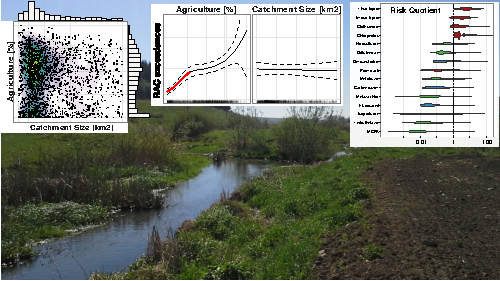
\includegraphics[width=0.7\textwidth]{abstract.pdf}

\end{tocentry}


%%%%%%%%%%%%%%%%%%%%%%%%%%%%%%%%%%%%%%%%%%%%%%%%%%%%%%%%%%%%%%%%%%%%%
\begin{abstract}
% 150-200 words
Small streams are important refugia for biodiversity.
In agricultural areas, they may be at high risk of pesticide pollution. However, most related studies have been limited to a few streams on the regional level, hampering extrapolation to larger scales.
In Germany, pesticide monitoring is performed by the federal states as part of water quality surveillance. 
\end{abstract}


%% -------------------------------------------------------------------------
\section{Introduction}
More than 50\% of the total land area in Germany are used by agriculture \citep{statistisches_bundesamt_bodenflache_2014}.
In the year 2014 more than 45,000 tonnes of 766 authorized pesticides were sold for application on this area \citep{bundesamt_fur_verbraucherschutz_und_lebensmittelsicherheit_absatz_2015}.
The applied pesticides may enter surface waters via spray-drift, edge-off-field run-off or drainage \citep{stehle_probabilistic_2013,schulz_comparison_2001,liess_determination_1999}.
Especially run-off after heavy precipitation events has been shown to be one of the major input routes for pesticides \citep{schulz_field_2004}.
Once entered the surface waters they may have adverse effects on biota and ecosystem functioning \citep{schafer_thresholds_2012}. 
Although, it is known that pesticides pollution and its effect increase with agricultural land-use \todo{citation needed}, studies investigating the shape of this relationships are missing.

\citet{malaj_organic_2014} analyzed data supplied to the European Union (EU) in the context of the Water Framework Directive (WFD) and showed that most European water bodies are at risk from pesticides.
\citet{stehle_pesticide_2015} compiled 1566 measured concentrations of 23 insecticides in the EU from scientific publications. 
They found that many of these measurements exceed regulatory acceptable concentrations (RAC).
Both studies indicate that pesticides might be a threat to biodiversity in the European union. 
However, theses studies reflect only a small amount of data and it is unclear how representative they are:
For Germany the study of \citet{malaj_organic_2014} lists only 175 sites and \citet{stehle_pesticide_2015} only 138 measurements. %175 estimated from digitized figure C.3 in Malaj 2014, Stehle: Table 2.
National monitoring programs are setup for the surveillance of water quality.
In Germany these are setup independently by the federal states in compliance with the WFD \citep{quevauviller_water_2008} and additional state specific needs. 
These programs may provide the most comprehensive data that is currently available for pesticide occurrences in German rivers.
However, currently there is no curated national-wide compilation of this monitoring data available.

Small waters (SW) comprise a major fraction of streams \citep{nadeau_hydrological_2007}, accommodate a higher proportion of biodiversity compared to larger freshwater systems \citep{davies_comparison_2008, biggs_report_2014} and play an important role in recolonization of disturbed downstream reaches \citep{liess_analyzing_2005, orlinskiy_forested_2015}.
However, SWB might be also at high risk of pesticide contamination from adjacent agricultural areas and lower dilution potential \citep{schulz_field_2004}.
It has been shown that SW are more polluted than bigger streams \citep{stehle_pesticide_2015,schulz_field_2004}.
Despite their relevance only a small fraction of studies were conducted on pesticide pollution of SW \todo{citation Lorenz et al.}, with only few large scale studies.

In this study we try to fill this gap and analyze nation-wide chemical monitoring data from SWB from Germany.
Using this large scale dataset we aimed to answer the following research questions: 

\begin{enumerate}[(i)]
  \item Is currently available monitoring data suitable for a description of pesticide pollution?
	\item How does the relationship between agricultural land use and catchment size with pesticide pollution look like?
  Are there thresholds for where pesticide pollution becomes apparent?
  \item Are samples taken during or shortly after heavy rainfall events or different seasons more likely to indicate chemical pollution?
	\item  How polluted are SWB in Germany and which pesticides currently pose the biggest threat to them?
\end{enumerate}

Answering these questions might give important insights for future monitoring planning, ecological risk assessment and water resource management.




%% -------------------------------------------------------------------------
\section{Methods}
\subsection{Data compilation}
We compiled pesticide monitoring data from sampling sites with catchment sizes $\mathrm{< 100km^2}$ for the years 2005 to 2015 from all 13 non-city federal states of Germany (see supplemental table S1 for the abbreviations of federal state names). 
We homogenized and unified all data from the states into a common database.
We implemented a robust data cleaning workflow (see supplemental figure S1 for details on data processing) \citep{poisot_best_2015}.
Nevertheless, parts of the dataset are proprietary and cannot be shared here.

Given the relevance of precipitation in causing runoff events, we identified chemical samples taken during heavy rainfall events.
We performed a spatio-temporal intersection of sampling events with gridded daily precipitation data available the German Weather service.
This data spatially interpolates daily precipitation values from local weather stations \citep{rauthe_central_2013}. 
We performed the intersection for the actual sampling date and the day before.

\subsection{Characterization of catchments}
We compiled a total of 3,049 sampling sites with pesticide measurements.
We delineated catchments upstream for each of the sampling sites using a digital elevation model (DEM) \citep{eea_digital_2013} and the multiple flow direction algorithm \citep{holmgren_multiple_1994} as implemented in GRASS GIS 7 \citep{neteler_grass_2012}.
Catchment delineation was manually checked for accuracy by comparison with a stream network provided by the government.
The delineation algorithm produced only for 30\% of the sites accurate results.
For the rest we were able to compile catchment size data from authorities (47\% of sites) or drainage basins per stream segment provided by authorities (13\% of sites).
For 10\% of the sites we were not able to compile catchment size data.
For each derived catchment (either from DEM or drainage basins) we calculated the relative cover (in \%) with agricultural areas based on Official Topographical Cartographic Information System (ATKIS) of the land survey authorities \citep{adv_atkis_2016}.
We additionally used agricultural cover data provided by authorities (18\% of sites), which resulted to 21\% of sites with missing agricultural cover data. 
For 78\% of the sites both, the proportion of agricultural landuse and catchment size were available.
% see do_overview.R for numbers

\subsection{Characterization of chemical pollution}
We characterized pesticide pollution using regulatory acceptable concentrations (RAC) \citep{brock_linking_2010}.
RACs are derived during pesticide authorization and no unacceptable ecological effect are expected if the environmental concentration remains below this concentration.
The German Federal Environmental Agency provided RACs for the 105 compounds with highest detection rates (Supplement, Table S2). 
We expressed RACs as Risk Quotient (RQ):

\begin{equation}
RQ_i = \frac{C_i}{RAC_i}
\end{equation}

Where $C_i$ is the concentration of a compound $i$ in a sample.

\subsection{Statistical analyses}
All data-processing and analyses were performed using R \citep{r_core_team_r:_2016}.
To display differences in the spectra of analyzed compounds between federal states we used Multidimensional Scaling (MDS) based on Jaccard dissimilarity in conjunction with complete linkage hierarchical clustering using the vegan package \citep{oksanen_vegan:_2016}.
We expected non-linear responses to agriculture and catchment size and therefore, used generalized additive models (GAM) to identify relationships \citep{fewster_analysis_2000}.
We modeled the number of RAC exceedances (RQ \textgreater 1) as:

\begin{align}
\begin{split}
  No_i \sim NB(\mu_i, \kappa) \\
  % E(No_i) = \mu_i~and~Var(No_i) = \mu_i + \frac{\mu_i^2}{\kappa} \\
  log(\mu_i)= \beta_0 + f_1(Agri_i) + f_2(Size_i) + log(n_i) \\
\end{split}
\end{align}

where $No_i$ is the observed number of exceedances at site $i$. 
We modeled $No_i$ as resulting from a negative binomial distribution ($NB$).
The proportion of agriculture within the catchment ($Agri_i$) and the catchment size of the site ($Size_i$) were used as predictors. 
$f_1$ and $f_2$ are smoothing functions using penalized cubic regression splines \citep{wood_generalized_2006}.
The degree of smoothness was estimated using restricted maximum likelihood (REML) during model fitting process \citep{wood_fast_2011}.
The number of sampling events per site ($n_i$) was used as an offset to account different sampling efforts at a site and is equivalent to modeling the rate of exceedances. 
We used point-wise 95\% Confidence Intervals (CI) of the first derivative of the fitted smooth to check if there are regions of statistically significant changes.
GAMs were fitted using the mgcv package \citep{wood_fast_2011}.

\todo{Überleitung}
RQ showed a skewed distribution with an excess of zeros (no pesticides with RAC detected). 
Therefore, we modeled these as two processes (one generating values below the limit of quantification (LOQ) and one generating values above LOQ) using a Zero-Adjusted Gamma (ZAGA) distribution \todo{Cite rigby 2010}:

\begin{align}
y \sim ZAGA(\mu, \pi) = 
  \begin{cases}
    (1 - \pi)   & \quad  \text{if } y < LOQ \\
    \pi \times f_{Gamma} (\mu) & \quad \text{if } y > LOQ \\
  \end{cases}
  \label{eqn:eqn3}
\end{align}

$\pi$ denotes the probability of a observation being above LOQ and $f_{Gamma}$ denotes the gamma function and is used for values greater LOQ.
We used the precipitation at sampling date ($prec_0$) and the day before ($prec_{-1}$), as well as quarters of the year ($season_{Q1-Q4}$) as linear predictors for the mean RQ ($\mu$) and the $\pi$:

\begin{align}
\begin{split}
\log(\mu) = \beta_0 + \beta_1 \times prec_0 + \beta_2 \times prec_{-1} + \beta_{3-5} \times season_{Q2-Q4} \\
logit(\pi) = \beta_0 + \beta_1 \times prec_0 + \beta_2 \times prec_{-1} + \beta_{3-5} \times season_{Q2-Q4} \\
\end{split}
\label{eqn:eqn4}
\end{align}

Changes in $\mu$ can be interpreted as changes in the absolute value of RQ, whereas changes in $\pi$ can be interpreted as changes in the probability that there is any risk.
To account for temporal autocorrelation and differences between federal states we used the site nested within state as random factors.
We fitted this model separatedly to each compound with a RAC, with at least 500 samples and more then 5\% of values above quantification limit.

\todo{check formulas, add i, add random effect? }

\todo{1 - remove columns from appendix table, 
2- keep only those with RACs,
3- indicate which where used for modeling here
}



\todo{Add definition of swb.}

%% -------------------------------------------------------------------------
\section{Results}
\subsection{Overview of the compiled data}

The compiled dataset comprised only few standing waters (58 sites) and the majority of samples (91\%) where taken via grab sampling.  % see clean.R for numbers
9\% of samples from 33 sites were taken as composite samples of different durations.
Therefore, we restricted the analyses to grab samples from streams. 
The analyzed dataset comprised 2,918,604 pesticide measurements of 42,236 samples in 3,049 sampling sites.  %see do_overview.R for numbers.
We found large differences in the number of sampling sites between federal states (Figure \ref{fig:fig1} and Supplement, Table S1).

\begin{figure}[ht]
  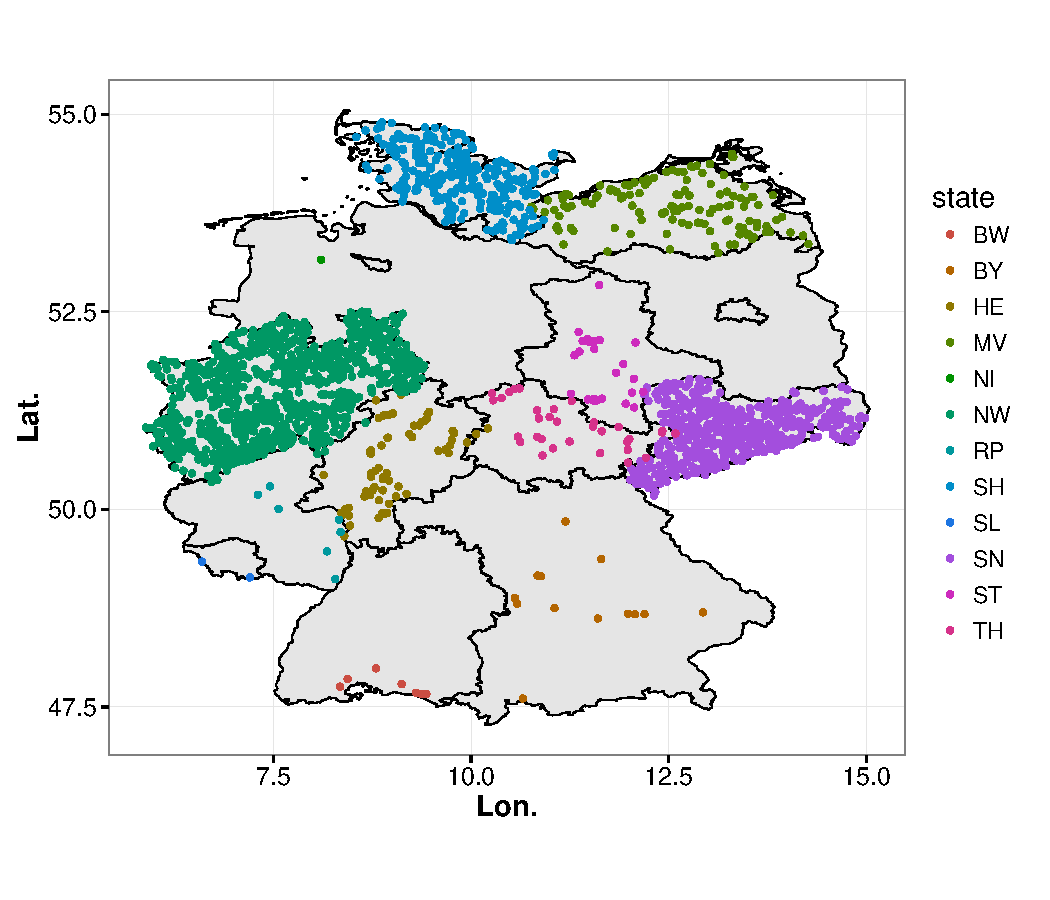
\includegraphics[width=0.6\textwidth]{figure1.pdf}
  \caption{Spatial distribution of the 3109 sampling sites. Colour codes different federal states, see supplemental table S1 for abbreviations.}
  \label{fig:fig1}
\end{figure}

In total 484 different compounds used as pesticides and their metabolites were measured at least once (Supplement, Table S2 \todo{remove LC50 and MAC-EQS from table!}). 
Most of the compounds were herbicides (179), followed by insecticides (117) and fungicides (109).
Most samples were take in the months April till October, with less samples in the winter (see Supplemental Figure S2).
Only 5.5\% (160,800) of all measurements were detects above the limit of quantification (LOQ).
We found substantial differences in the spectra of analyzed compounds between federal states (Figure \ref{fig:fig2}).
Hierarchical clustering revealed three groups (see also Supplement Figure S2):

\begin{enumerate}[i)]
	\item with less then 100 compounds (SL, ST and TH)
	\item with medium sized spectra
	\item with a big and distinct spectrum (RP and NI)
\end{enumerate}

\begin{figure}[ht]
  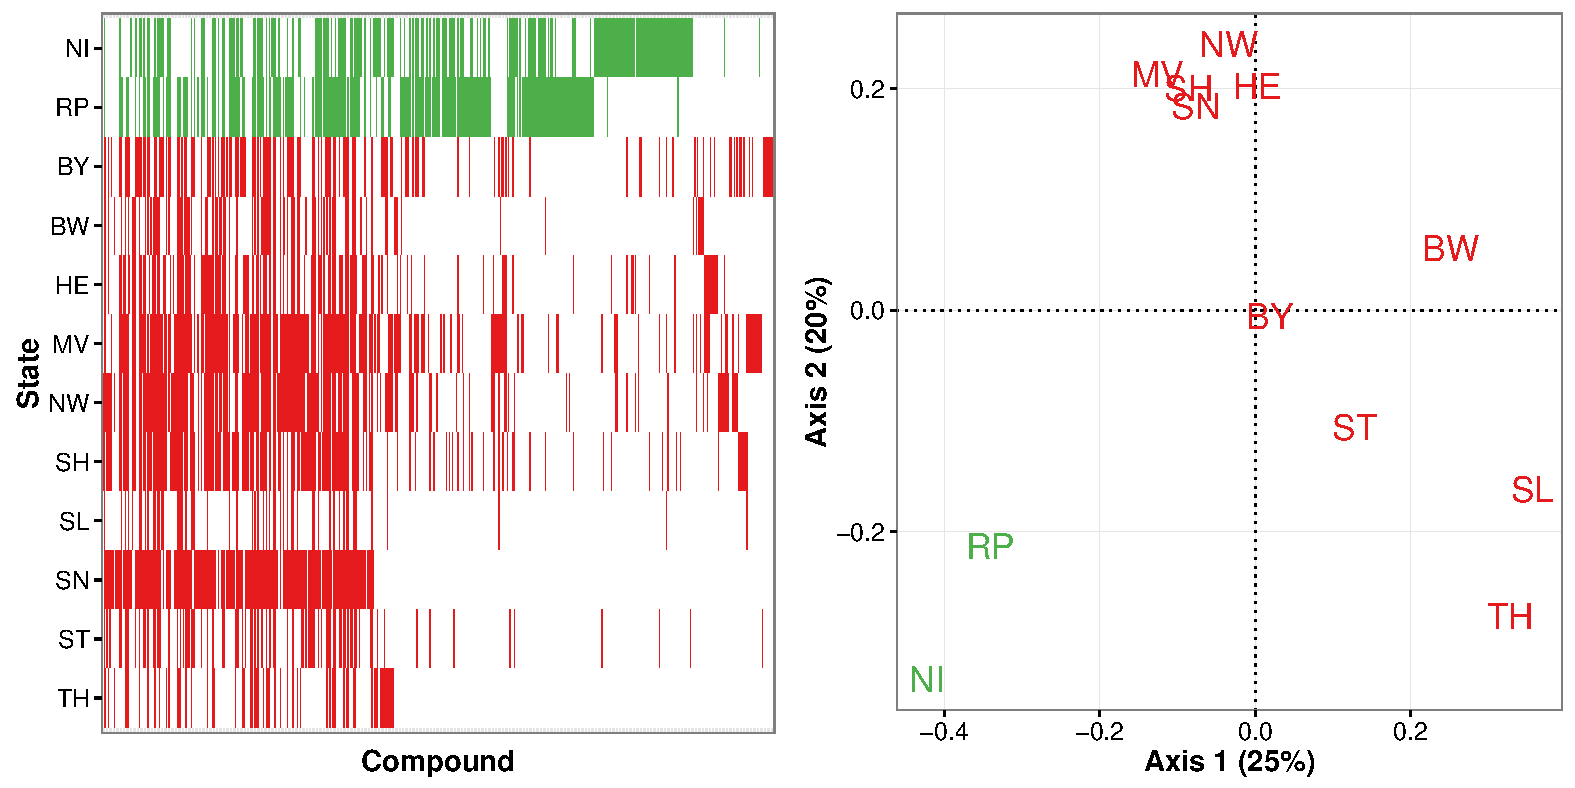
\includegraphics[width=\textwidth]{figure2.pdf}
  \caption{Compound spectra of the different federal states. Left: Barcode plot - each vertical line is an analysed compound. Right: MDS ordination. 
  Colors according to three groups determined by hierarchical clustering (see Supplement Figure S2).}
  \label{fig:fig2}
\end{figure}

The distribution of sampling sites across catchment area and agricultural area in the catchment revealed a sharp decline in the distribution of catchment-sizes below $10~km^2$, with most sampling sites with catchments between 10 and 25 $km^2$ (Figure \ref{fig:fig3}).
The proportion of agriculture in the catchments decreased with increasing catchment size.

\begin{figure}[ht]
  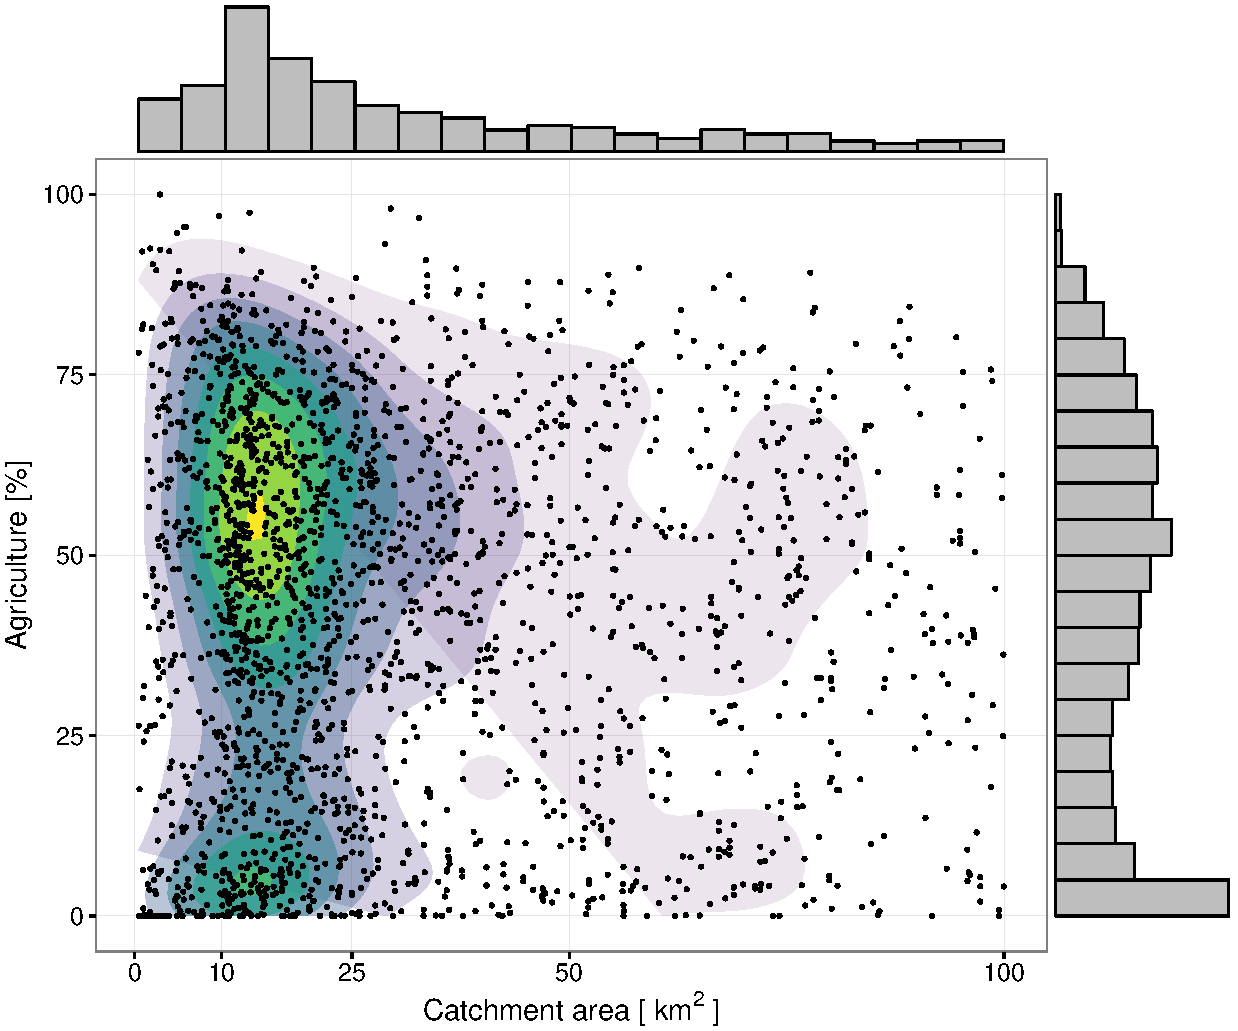
\includegraphics[width=.8\textwidth]{figure3.pdf}
  \caption{Distribution of catchment area and agriculture within the catchment area across the sampling sites.
  Only sampling sites with catchment area < 150 km\textsuperscript{2} are displayed. 
  Colour codes the 2-dimensional density of points.}
  \label{fig:fig3}
\end{figure}



\subsection{Thresholds for agricultural land use and catchment size}
Modeling the number of RAC exceedances as function of agriculture within catchment and catchment size revealed that there is a strong and statistically significant increase up to 25\% agriculture.
Above this threshold the exceedances level off followed by a increase above 75\% (Figure \ref{fig:fig4}, left).
We could no detect any effect of catchment size on the number of RAC exceedances (Figure \ref{fig:fig4}, right).
We also found no statistically significant interaction between catchment size and agriculture.

\begin{figure}[ht]
  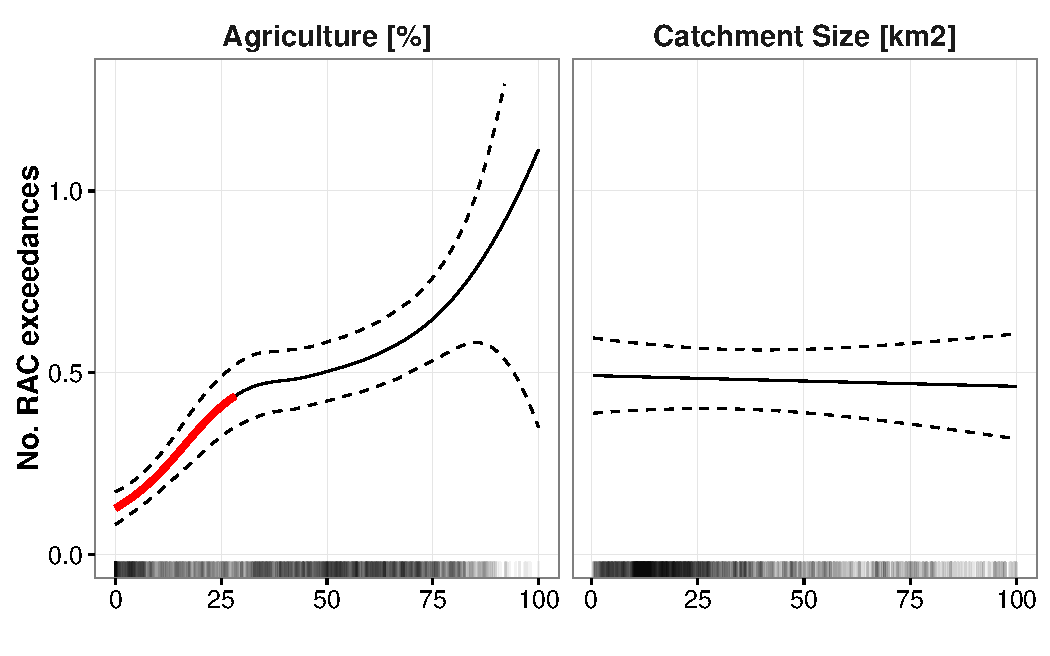
\includegraphics[width=0.95\textwidth]{figure4.pdf}
  \caption{Effect of agriculture within the catchment (left) and catchment size (right) on the number of RAC exceedances. Red line marks statistically significant changes. Dashed lines denote 95\% pointwise Confidence Intervals.
  }
  \label{fig:fig4}
\end{figure}



\subsection{Effect of precipitation on exposure}

The spatio-temporal intersection revealed that 5\% of the samples were taken at or after days with rainfall events greater than 10mm / day (Supplement, Figure S3).

\begin{figure}[ht]
  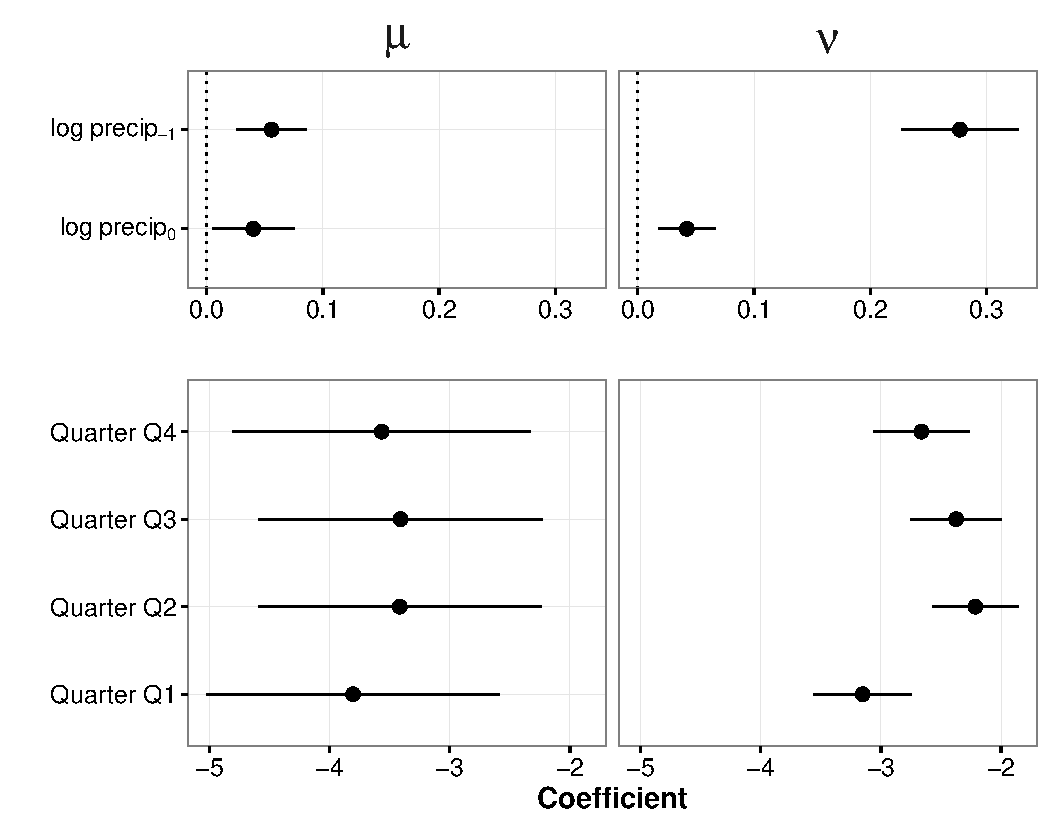
\includegraphics[width=0.95\textwidth]{figure5.pdf}
  \caption{Estimated coefficients and their 95\% CI for the model describe in equations \ref{eqn:eqn3} and \ref{eqn:eqn4}. Left column: Effect on mean RQ; Right column: effect on the probability that RQ \textgreater 0.
  Coefficient where the CI does not encompasses zero are shown in black.
  }
  \label{fig:fig5}
\end{figure}

\subsection{Pesticide pollution of small water bodies}




\section{Discussion}
\subsection{Overview on the compiled dataset}
The compiled dataset of governmental monitoring data represents currently the most comprehensive one available for Germany.
Similar nationwide datasets have been compiled for the Netherlands \citep{vijver_spatial_2008}, Switzerland \citep{munz_pestizidmessungen_2011} and the United States (Water Quality Portal (WQP) \url{www.waterqualitydata.us}).
The data compiled and analysed here for Germany is of similar quantity and quality.










%%%%%%%%%%%%%%%%%%%%%%%%%%%%%%%%%%%%%%%%%%%%%%%%%%%%%%%%%%%%%%%%%%%%%
\begin{acknowledgement}
The authors thank the federal state authorities for providing chemical monitoring data and the German Federal Environmental Protection Agency (UBA) for funding a related project (FKZ 3714 67 4040 / 1). 
\end{acknowledgement}


%%% Word count
% abstract    :
% 3 big(600)  : 1800
% 2 small(300): 600
% text body   : 3000 
% ackno       : 24
% ======================================
% total       : 

%%%%%%%%%%%%%%%%%%%%%%%%%%%%%%%%%%%%%%%%%%%%%%%%%%%%%%%%%%%%%%%%%%%%%
\begin{suppinfo}
The following files are available free of charge.
\begin{itemize}
  \item Supplemental\_Materials.pdf : Supplemental Materials (Figures, Tables, Models).
\end{itemize}
\end{suppinfo}


%%%%%%%%%%%%%%%%%%%%%%%%%%%%%%%%%%%%%%%%%%%%%%%%%%%%%%%%%%%%%%%%%%%%%
\bibliography{references}

\end{document}
